\section{Results}

Data was collected on the trajectories of the eleven subjects from the lowest stair configuration (config0). Eight subjects were randomly selected to train the model. The remaining three subjects were used for validation. No additional prepossessing of the mocap data was required except for the gap-filling done in the Vicon Nexus software. 

\autoref{fig:ytraj} and \autoref{fig:ztraj} compare the $Y$ and $Z$ positions of the right leg's toe marker for the eight validation subjects. Each of the trajectories shown in these graphs was input as a training demonstration for the model. Each of the subjects climbed at different speeds, but follow a similar trajectory. The trajectories were aligned using Dynamic Time Warping to solve the speed inconsistency, this scaling removed the time dependencies of the trajectories. This is shown in the time-normalized variable $s$, where $s$ 0 $\rightarrow$ 1. A temporally-scaled trajectory is not continuous; the trajectories contain jagged segments and are thus not differentiable. A high order polynomial smoothed each warped trajectory to ensure that it is continually differentiable. The $Y$ trajectories have different ending positions; this can be accounted for by the subject's different gaits. This variation allows the model to adapt. In addition, using DMPs allows for the abstraction of the goal. The trajectories can be scaled in time using the $\tau$ parameter. When $\tau$ is 1, the trajectory is reproduced in real time. To speed up the system, increase $\tau$ above 1. To slow it down, decrease it to less than 1.  

\begin{figure}[h]

    \begin{subfigure}{\linewidth}
        \centering 
        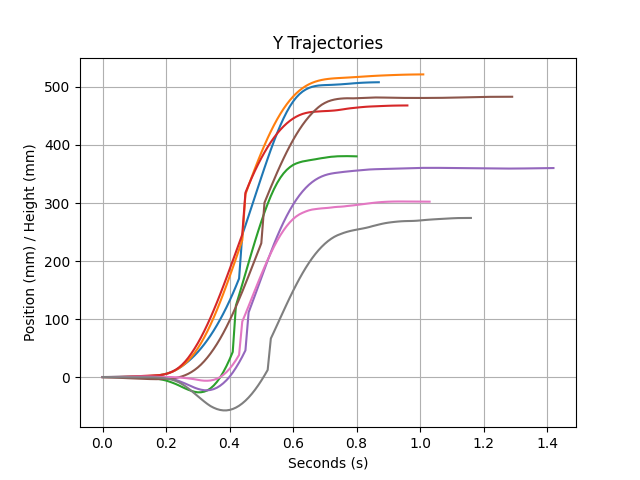
\includegraphics[ scale=0.5]{images/ytraj_s.png} 
        \caption{The toe marker $Y$ position trajectories} 
        \label{fig:ytraj} 
    \end{subfigure} 

    \begin{subfigure}{\linewidth}
        \centering 
        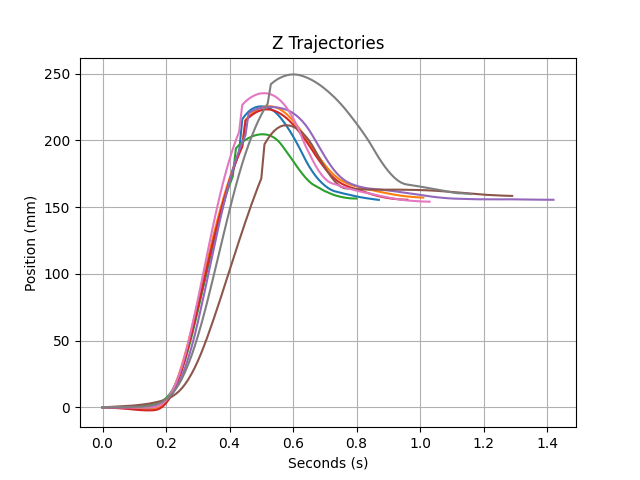
\includegraphics[ scale=0.5]{images/ztraj_s.png} 
        \caption{The toe marker $Z$ position trajectories} 
        \label{fig:ztraj} 
    \end{subfigure} 
    \caption{Comparison of different subjects' climbing motion in the sagittal plane. Each line is the motion from a different subject's trial.}
    \label{fig:trainingDemos}
\end{figure}

\autoref{fig:DTW} shows the alignment of a trajectory against a demonstration. The blue line is demo 1, and the orange line is demo 2. DTW aligns demo 2 with demo 1. The green line represents the aligned trajectory and the red line represents a polynomial fit to the aligned trajectory. The cost map shows the closest fit of points from $P$ to $T$. The white spots are the hills and the black spots are the valleys, with the path being the minimum cost from start to goal. The total path cost associated with the Euclidean was $17652.35$, and the cost of the Manhattan path was $33.50$. This is the cost of aligning the demonstration with the model trajectory. The Manhattan metric had a much lower cost than the Euclidean metric, allowing for a better fit. 



% \begin{figure} [h]
%     \centering 
%     \includegraphics[frame, scale=0.5]{images/ytraj.png} 
%     \caption{Subject Y Trajectories} 
%     \label{fig:ytraj} 
% \end{figure} 

% \begin{figure} [h]
%     \centering 
%     \includegraphics[frame, scale=0.5]{images/ztraj.png} 
%     \caption{Subject Z Trajectories} 
%     \label{fig:ztraj} 
% \end{figure} 


\begin{figure}[h]
     \centering 
     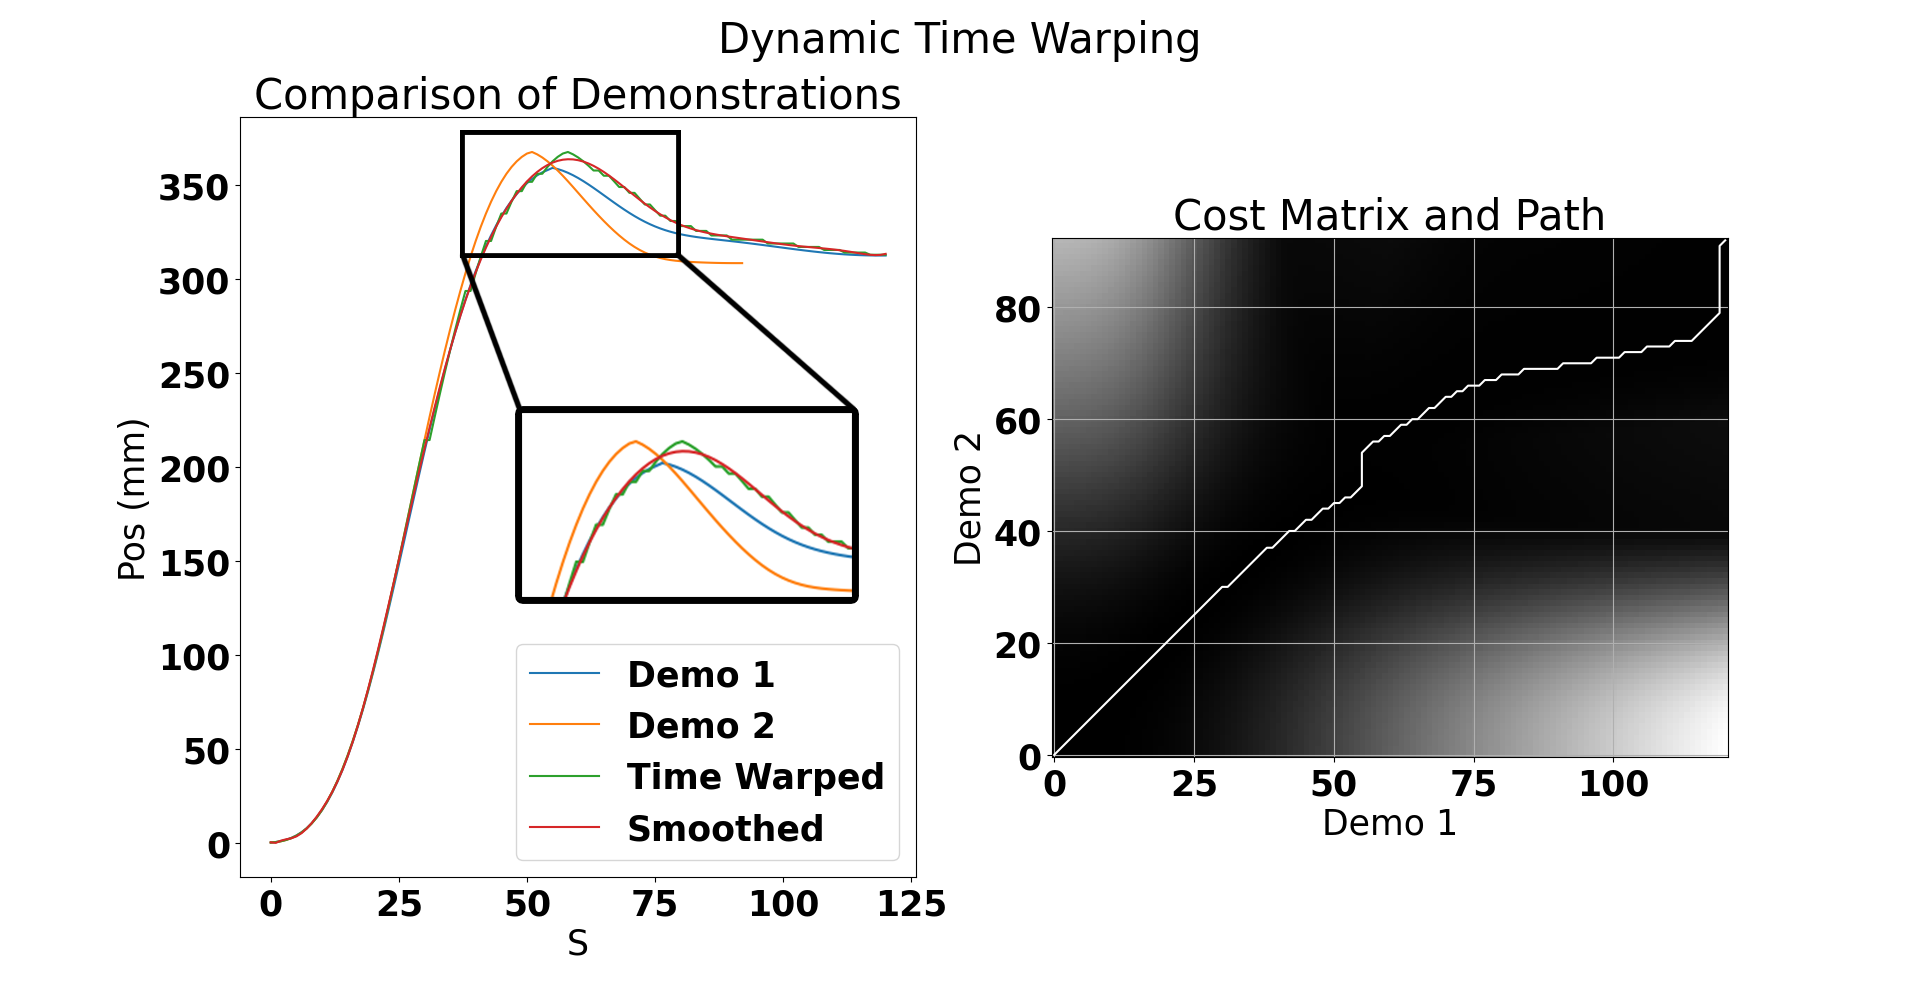
\includegraphics[ scale=0.12]{images/DTW_annotated.png} 
     \caption{Two demos being aligned using DTW and a smoothed trajectory. Blue line: demo 1. Orange line: demo 2. Green line: aligned trajectory. Red line: Polynomial smooth trajectory. The cost map shows the distance between the points.} 
     \label{fig:DTW} 
       \vspace*{-4mm}
\end{figure} 
 
\autoref{fig:BIC} shows the BIC score calculated for several bin sizes (1-24) for the $ Y $ and $ Z $ trajectories of the toe marker. This calculation limits the number of bins. The two graphs are generated using a single demonstration from each of the eight subjects in the config0 data set. The optimal number of bins for the $Z$ axis is 6 bins and the optimal number of bins for the $Y$ axis is 7 bins.


\begin{figure}[h]
   \begin{subfigure}{\linewidth} 
    \centering 
    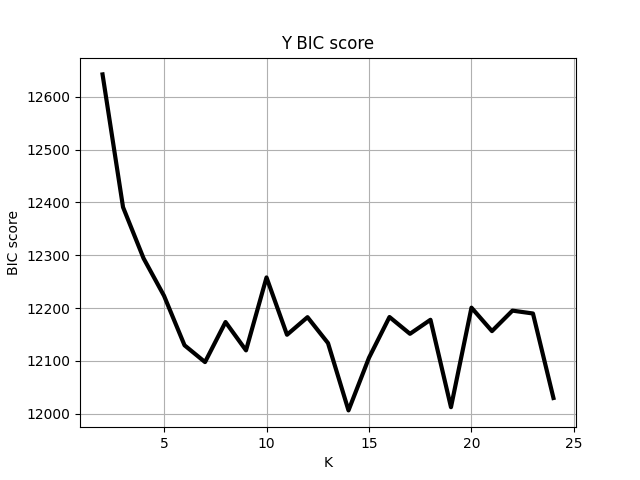
\includegraphics[ scale=0.48]{images/ybic7.png} 
    \caption{BIC score for toe marker $Y$ position trajectory. The BIC score has its first local minimum at a size of 7 bins.} 
    \label{fig:BICY} 
  \end{subfigure}  

   
\begin{subfigure}{\linewidth} 
    \centering 
    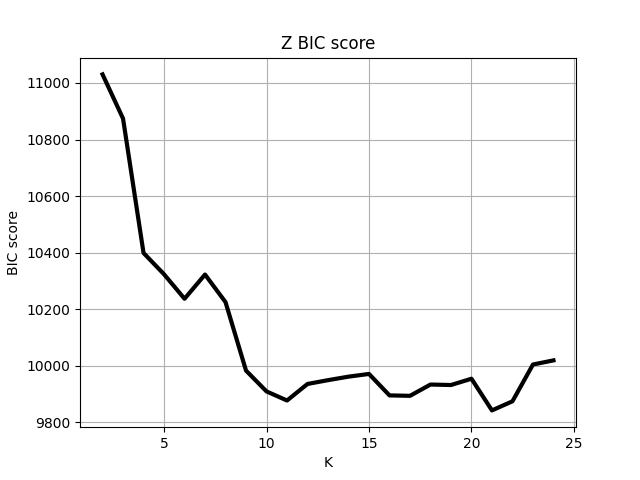
\includegraphics[ scale=0.48]{images/zbic6.png} 
    \caption{BIC score for toe marker $Z$ position trajectory. The BIC score has its first local minimum at a size of 6 bins.} 
    \label{fig:BICZ} 
  \end{subfigure}  
    \caption{The BIC score (smaller is better) was calculated for numerous bins size for the $Y$ and $Z$ trajectory.} 
    \label{fig:BIC} 
      \vspace*{-5mm}

\end{figure}  


\autoref{fig:GMM} shows the placement of the Gaussian on the learned forcing function for the $Z$ axis. Only one axis is reported to illustrate how the underlining model is created. The blue lines are the demonstrations of forcing functions and the yellow line is the learned forcing function. The green ovals are the Gaussian, and the red dots are the means of the Gaussian. This graph shows the areas of correlation among the demonstrations. The location of the Gaussian was determined by the EM step in the GMM algorithm, and the yellow line is the forcing function calculated by the GMR algorithm that regresses the Gaussian.    



\begin{figure}[h]
    \centering 
    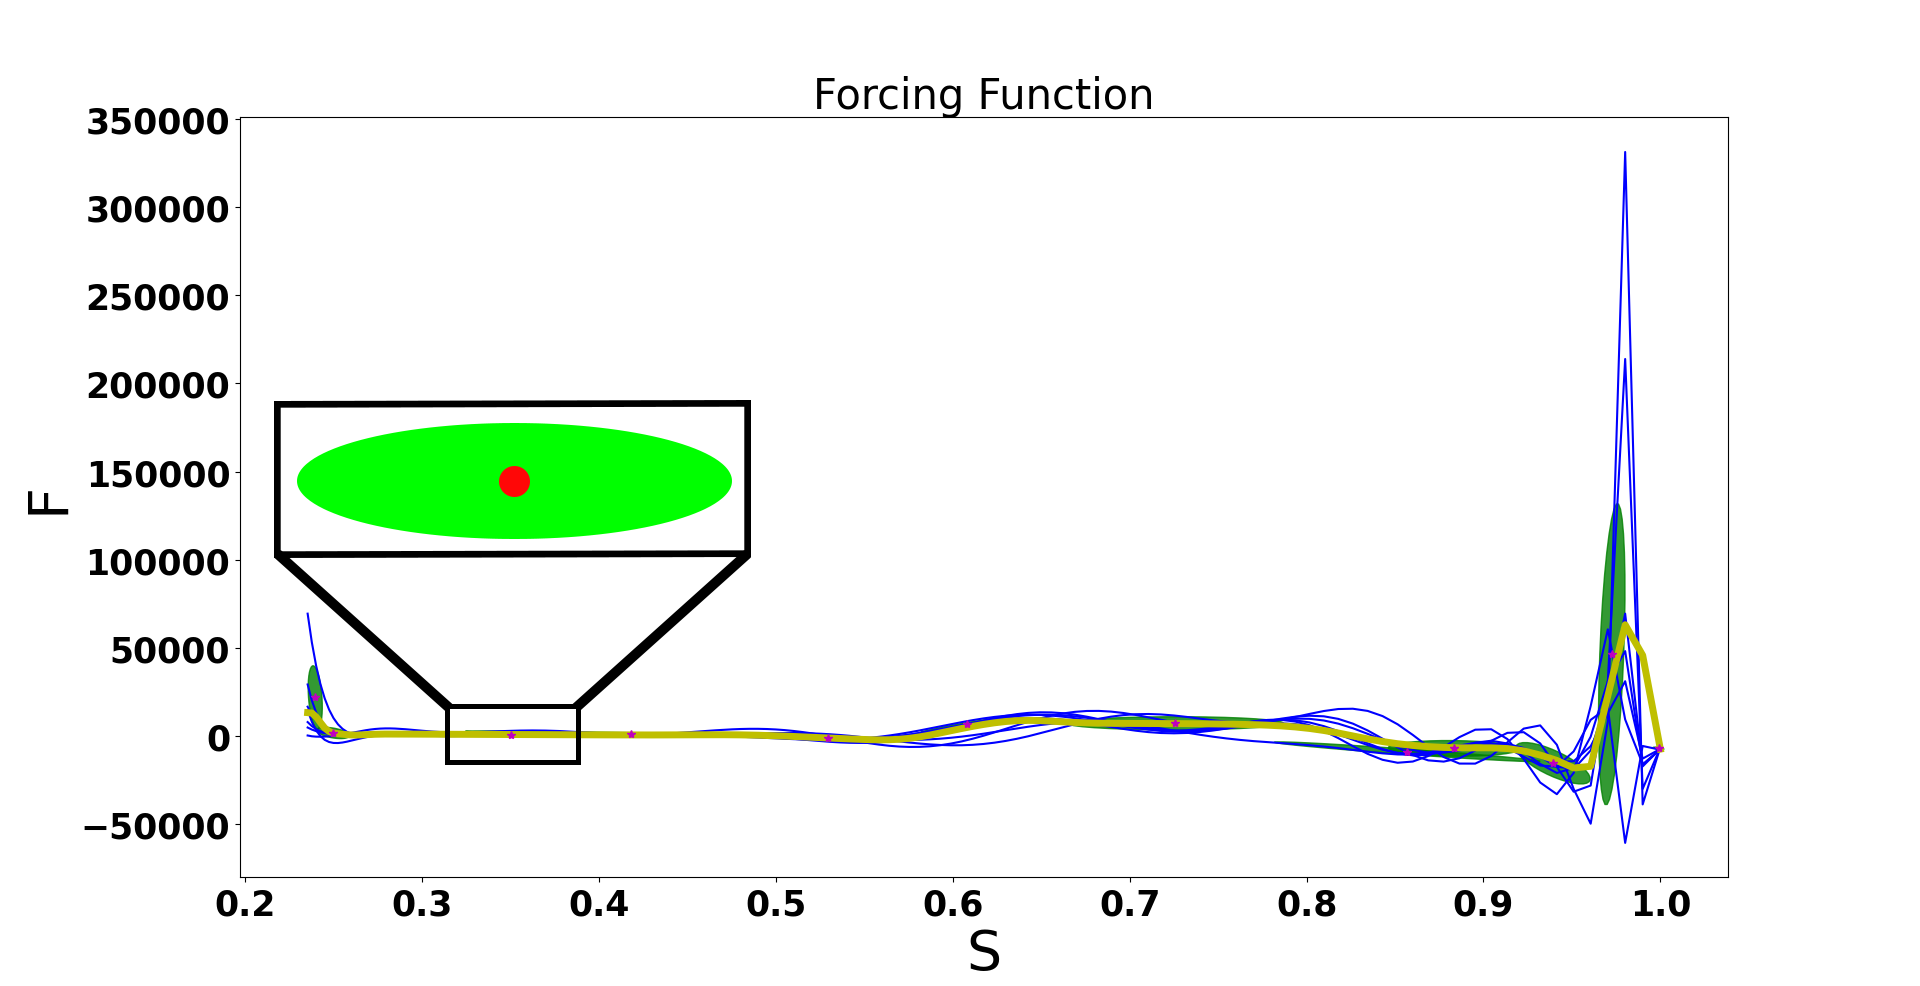
\includegraphics[ scale=0.13]{images/forcing_func_large.png} 
    \caption{The Gaussian positions over the demonstrations and the learned forcing function for the $Z$ axis. The blue lines are the demonstrations, the yellow line represents the learned mode, and the Gaussian is in the green ovals with the red dot as the mean of the Gaussian. The figure shows a zoomed-in Gaussian for comparison.} 
    \label{fig:GMM} 
\end{figure} 


\autoref{fig:trajLearning} shows the result of the learning of the $Y$ and $Z$ models using config0 subject data. The thick lines represent the generated model that was learned from the demonstrations using the optimal number of bins and demonstrations. The oscillations are caused by the DTW fitting of the demonstrations and the polynomial smoothing. The demonstrations with few points are being fit to the models with more points. The polynomial fitting ensures that the trajectories are smooth and not jagged.


\begin{figure}[h] 
  \centering 
  \begin{subfigure}{\linewidth} 
    \centering 
    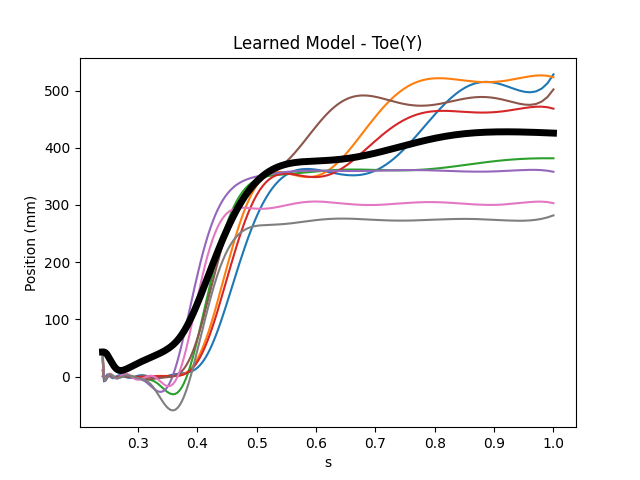
\includegraphics[ scale=0.50]{images/ylearn7.png} 
    \caption{Comparison of learning the $Y$ marker position trajectory} 
    \label{fig:compY} 
  \end{subfigure} 
  \begin{subfigure}{\linewidth} 
    \centering 
    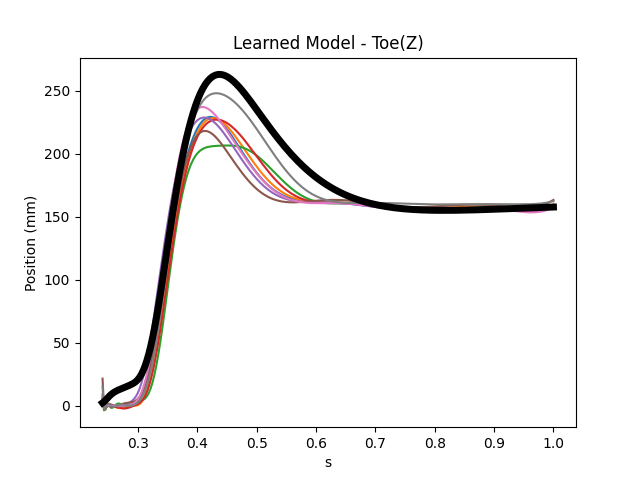
\includegraphics[ scale=0.50]{images/zlearn6.png} 
    \caption{Comparison of learning the $Z$ marker position trajectory} 
    \label{fig:compZ} 
  \end{subfigure}   
  \caption{Imitation model for the toe position for climbing a stair. The $Z$ position is height of the toe relative to the floor and the $Y$ position is where the toe lands relative to the body. The thick line is the imitation model. The models used the optimized number of bins calculated from the BIC score.} 
  \label{fig:trajLearning} 
    \vspace*{-2mm}
\end{figure}   


\autoref{fig:compare_methods} shows an example trajectory compared to that of a model trained from the motion of only a single subject and the model trained on all eight subjects. \autoref{tab:error} shows the imitation cost for a model trained with a single subject and a model trained using multiple subjects (see \autoref{eq:metric}). Both models were compared against a demonstration that was not used to train either model.  


% \begin{figure} 
%     \centering 
%     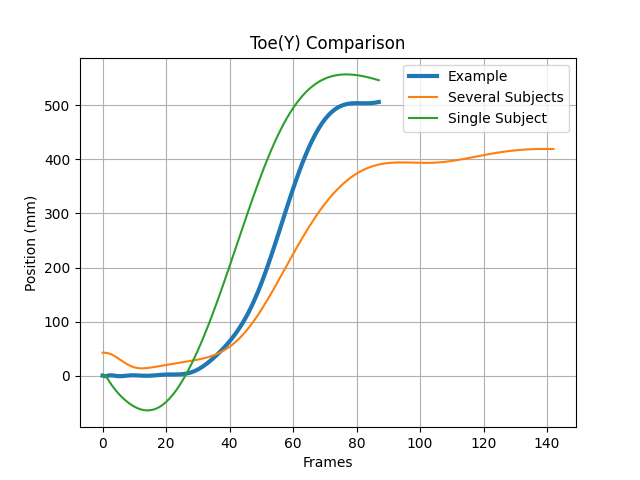
\includegraphics[frame, scale=0.5]{images/compy.png} 
%     \caption{Multiple vs single examples for Toe(Y) trajectory} 
%     \label{fig:compare_methodsy} 
% \end{figure} 

% \begin{figure} 
%     \centering 
%     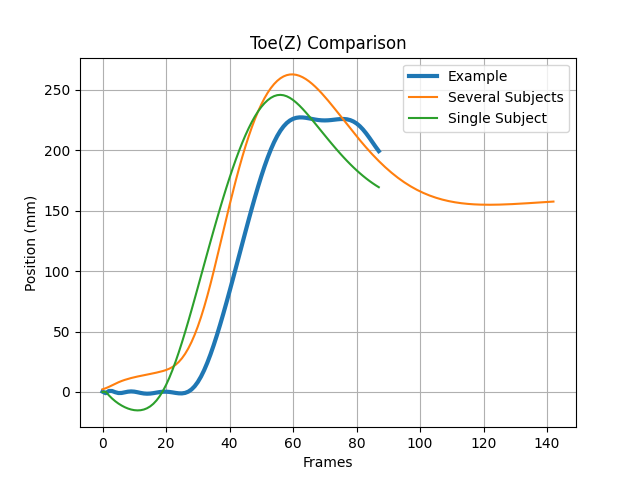
\includegraphics[frame, scale=0.5]{images/compz.png} 
%     \caption{Multiple vs single examples for Toe(Z) trajectory} 
%     \label{fig:compare_methodsz} 
% \end{figure} 

% \begin{figure}[h]
%     \centering
%     \begin{subfigure} {\linewidth} 
%         \centering 
%         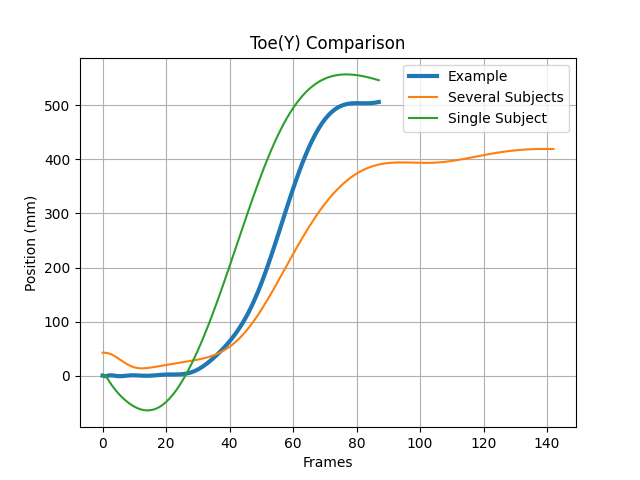
\includegraphics[frame, scale=0.5]{images/compy.png} 
%         \caption{Multiple vs single examples for Toe(Y) trajectory} 
%         \label{fig:compare_methodsy} 
%     \end{subfigure} 
% 
%     \begin{subfigure} {\linewidth} 
%         \centering 
%         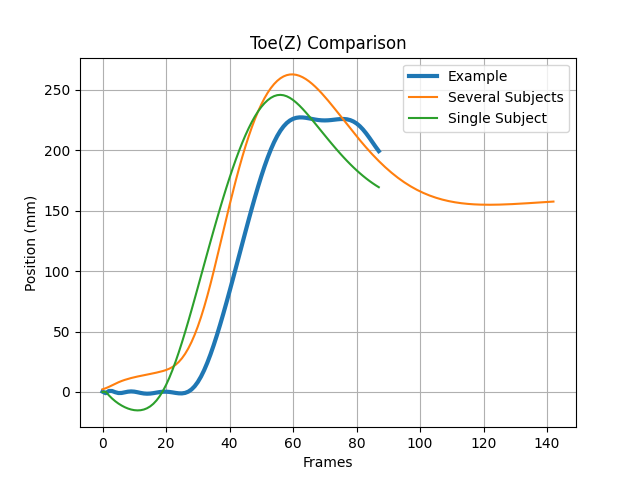
\includegraphics[frame, scale=0.5]{images/compz.png} 
%         \caption{Multiple vs single examples for Toe(Z) trajectory} 
%         \label{fig:compare_methodsz} 
%     \end{subfigure} 
%     \caption{Comparison of a demonstration against a model trained on a single demonstration and a model trained on multiple demonstrations.}
%     \label{fig:comparison}
% \end{figure}

\begin{figure}[h]
    \centering 
    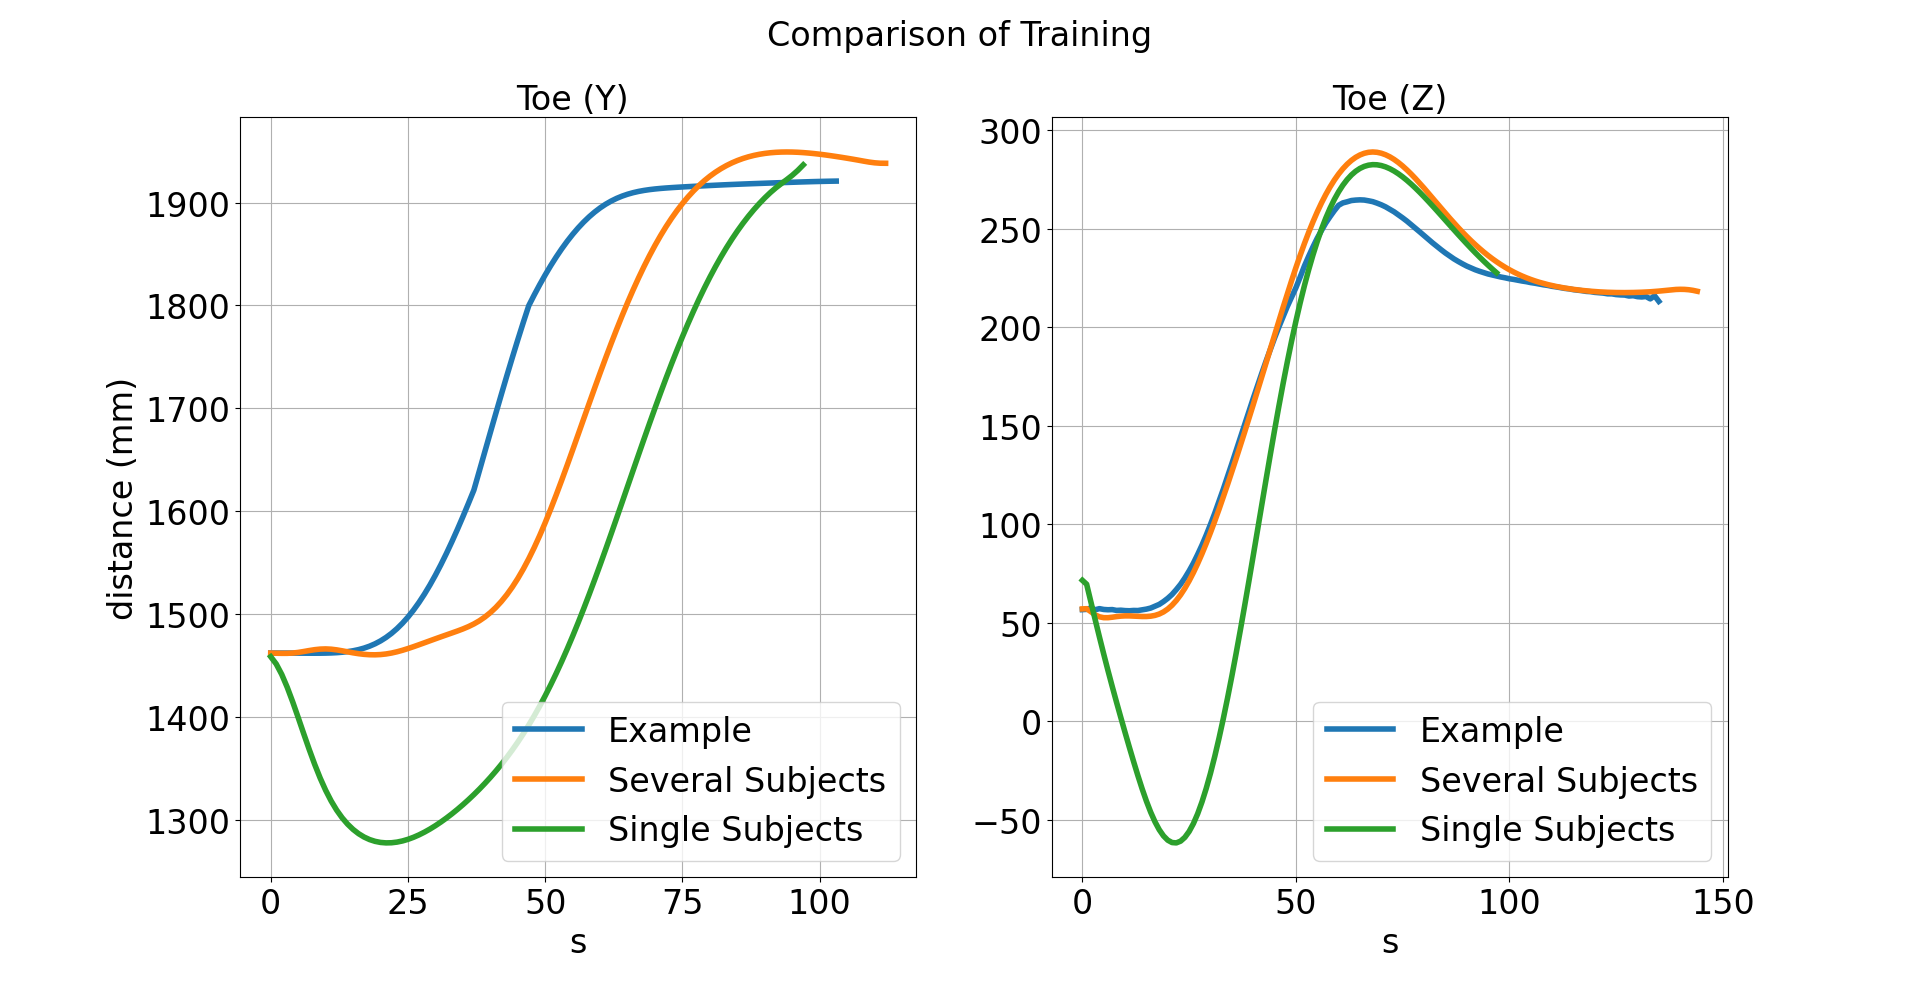
\includegraphics[scale=0.20]{images/compare_method.png} 
    \caption{Comparison of a demonstration against a model trained on a single demonstration and a model trained on multiple demonstrations. This is expressed over frames. } 
    \label{fig:compare_methods} 
\end{figure} 

\begin{table}[h]
\large 
     \centering 
     \begin{tabular}{||c|| c c ||}  
     \hline 
         Axis     & Y & Z  \\ [0.5ex]  
         \hline\hline 
         Single subject   & 138.01 & 67.86  \\  
         \hline 
         Multiple subjects & 70.7 & 25.63  \\ 
         \hline      
     \end{tabular} 
     \caption{Imitation cost (smaller is better) comparing models trained on a single subject to that trained on multiple subjects. The compared trajectories are shown in \autoref{fig:compare_methods}. } 
     \label{tab:error} 
\end{table} 


\autoref{fig:singleSubject} shows the training and reproduction of the models trained on different stair heights. The solid line is the raw trajectory, and the dotted line is the reproduced line. To test the model's ability to adapt to different stair heights, the goal($g$) of the model was changed to each of the different stair heights. For example, for the model trained on a trajectory whose end position (goal) was $250mm$, the goal was changed to a height of $275mm$. The model is able to follow a foot trajectory for a different stair height. This trajectory was not one of the demonstrations used to train the model.


\begin{figure}
    \centering
    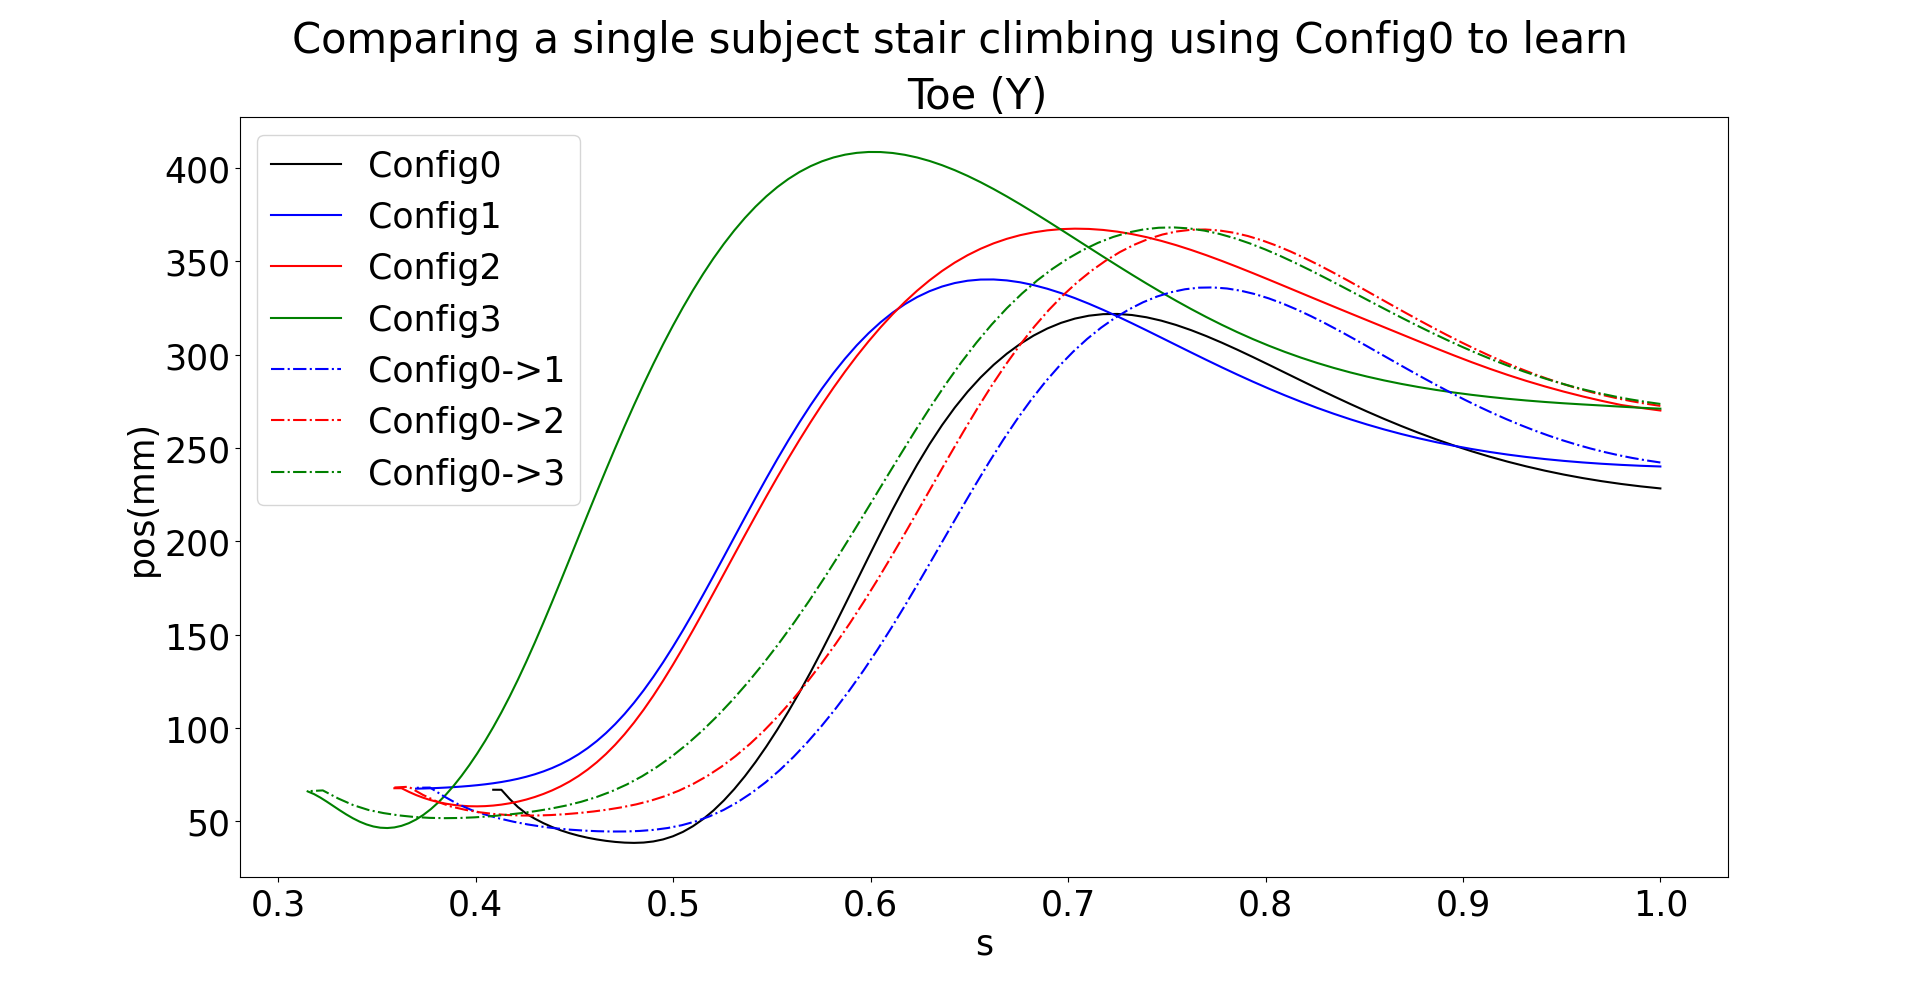
\includegraphics[scale=0.20]{images/compareHeihgts.png}
    \caption{A model trained on a single subject and single configuration, reproducing the motion climbing different stair heights. The solid lines are the marker trajectories. The dotted lines are the reproduced trajectories using the model.}
    \label{fig:singleSubject}
\end{figure}

% \begin{figure}[h]
%   \centering 
%   \begin{subfigure}{\linewidth} 
%     \centering 
%     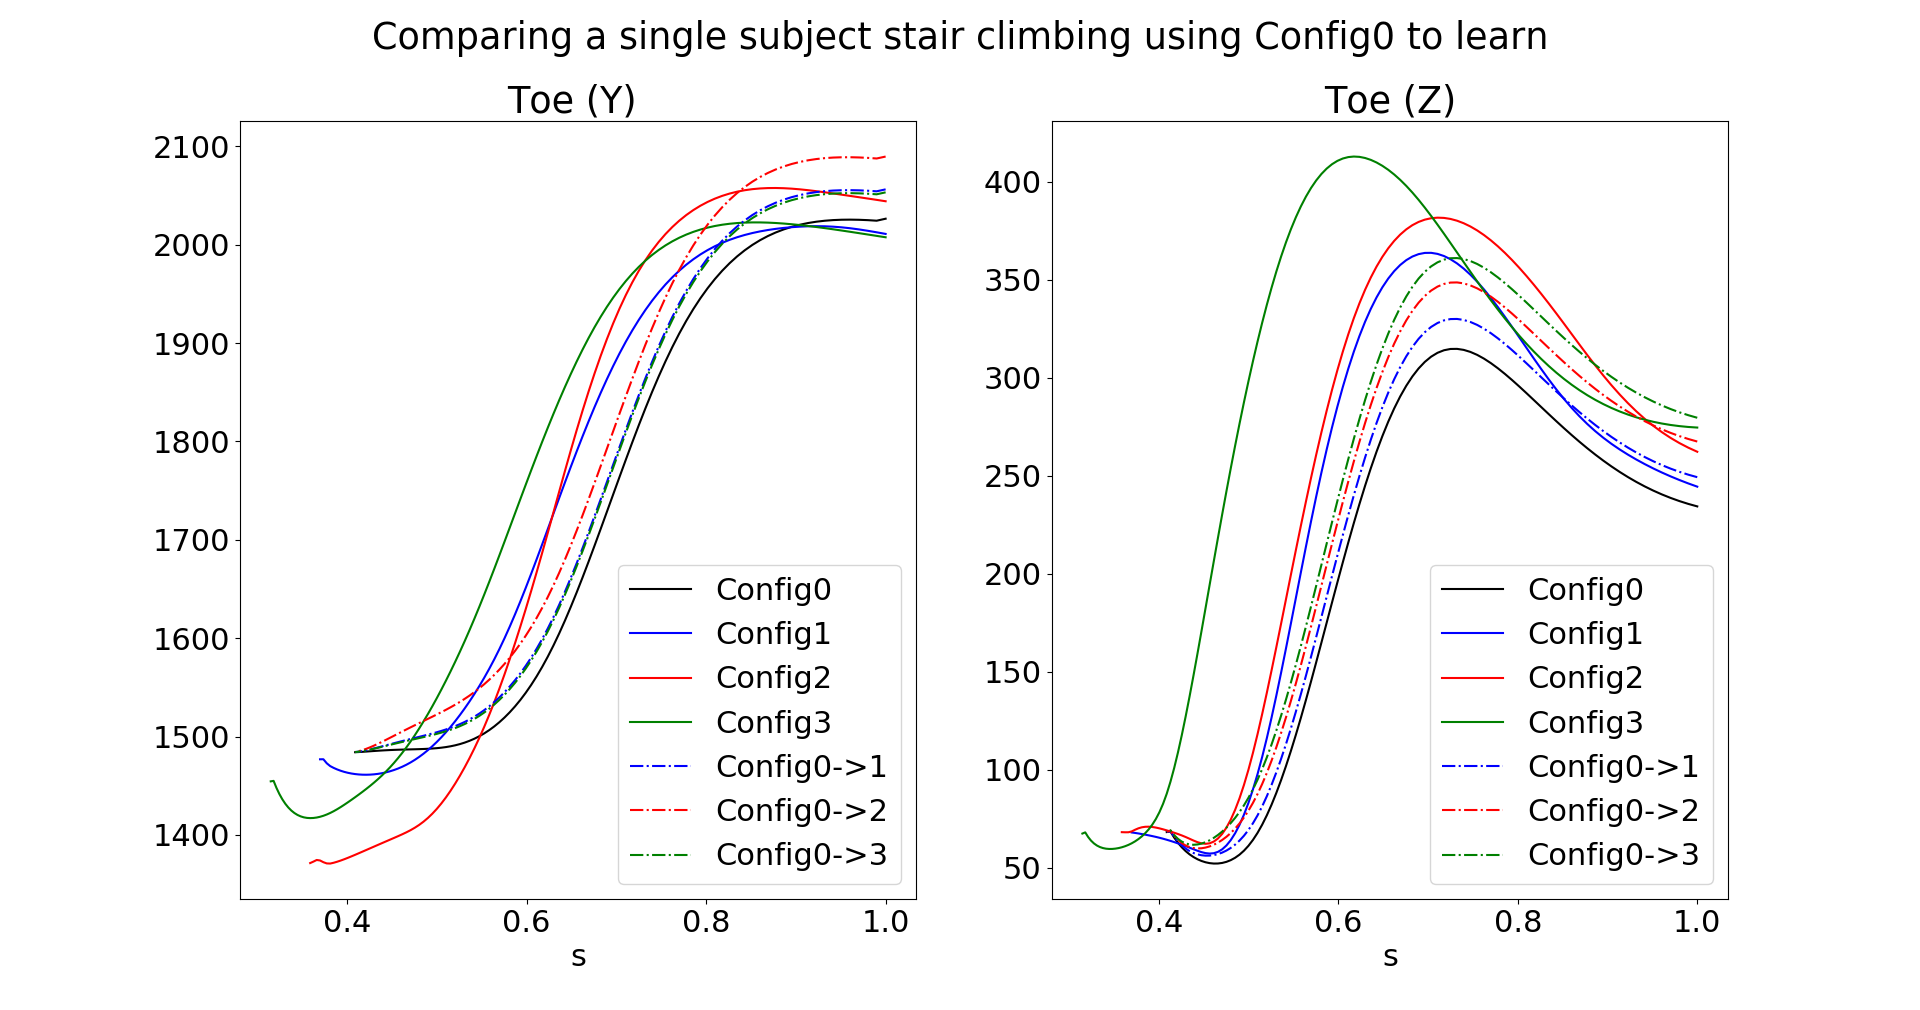
\includegraphics[frame, scale=0.17]{images/config0.png} 
%     \caption{Using config0 to learn} 
%     \label{fig:config0} 
%   \end{subfigure} 
%     \begin{subfigure}{\linewidth} 
%     \centering 
%     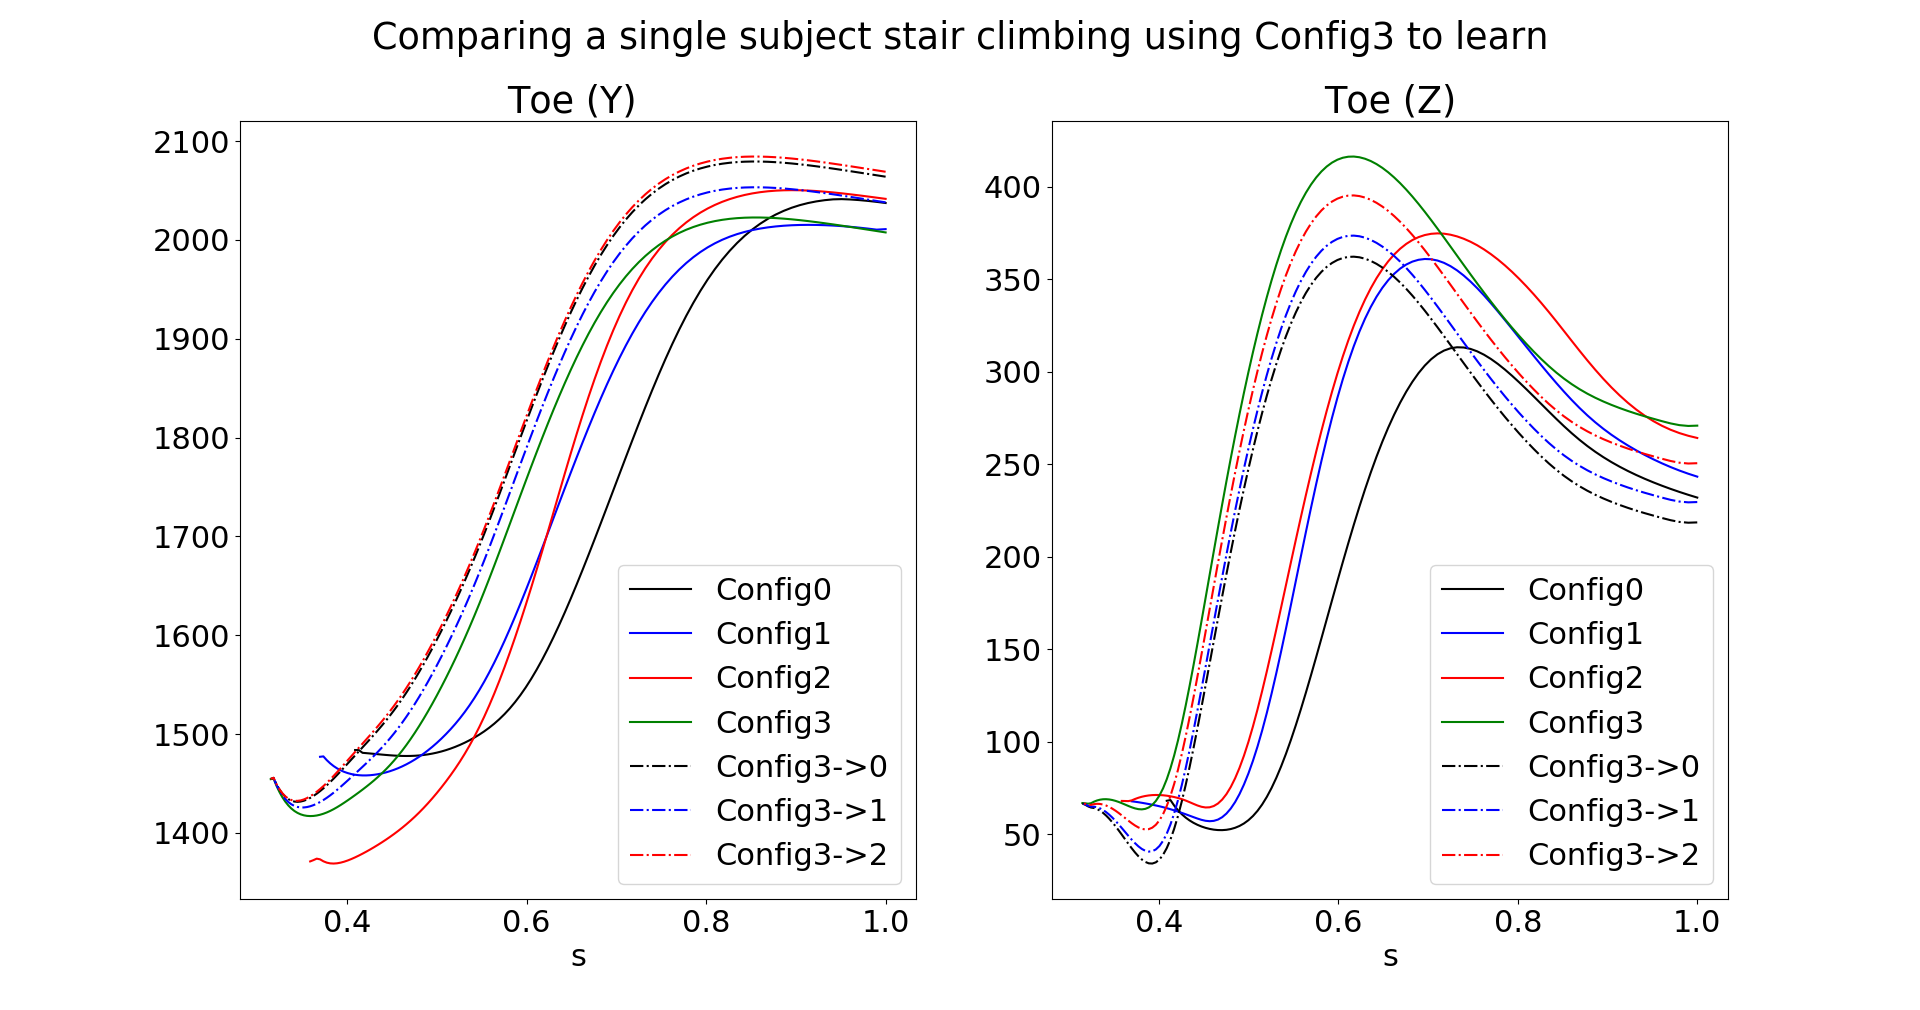
\includegraphics[frame, scale=0.17]{images/config3.png} 
%     \caption{Using config3 to learn} 
%     \label{fig:config3} 
%   \end{subfigure}   
%   \caption{A model trained on single subject and single configuration, reproducing the motion climbing different stair heights. The solid lines are the marker trajectories. The dotted lines are the reproduced trajectories using the model \autoref{fig:config3} that was trained on stair config3. The dotted lines should converge to the solid lines.} 
%   \label{fig:singleSubject} 
% \end{figure}   


Using the inverse kinematics and the anthropomorphic parameters, the joint angle can be calculated. \autoref{fig:stairsclimbing} shows the movement of the leg through a stepping trajectory. The trajectory of the toe is being controlled. The joint angles at each instance are determined using inverse kinematics. The ankle is constrained to be parallel to the ground. This constraint is to prevent the toe from catching on the edge of the stairs.


% \begin{figure}
%     \centering
%     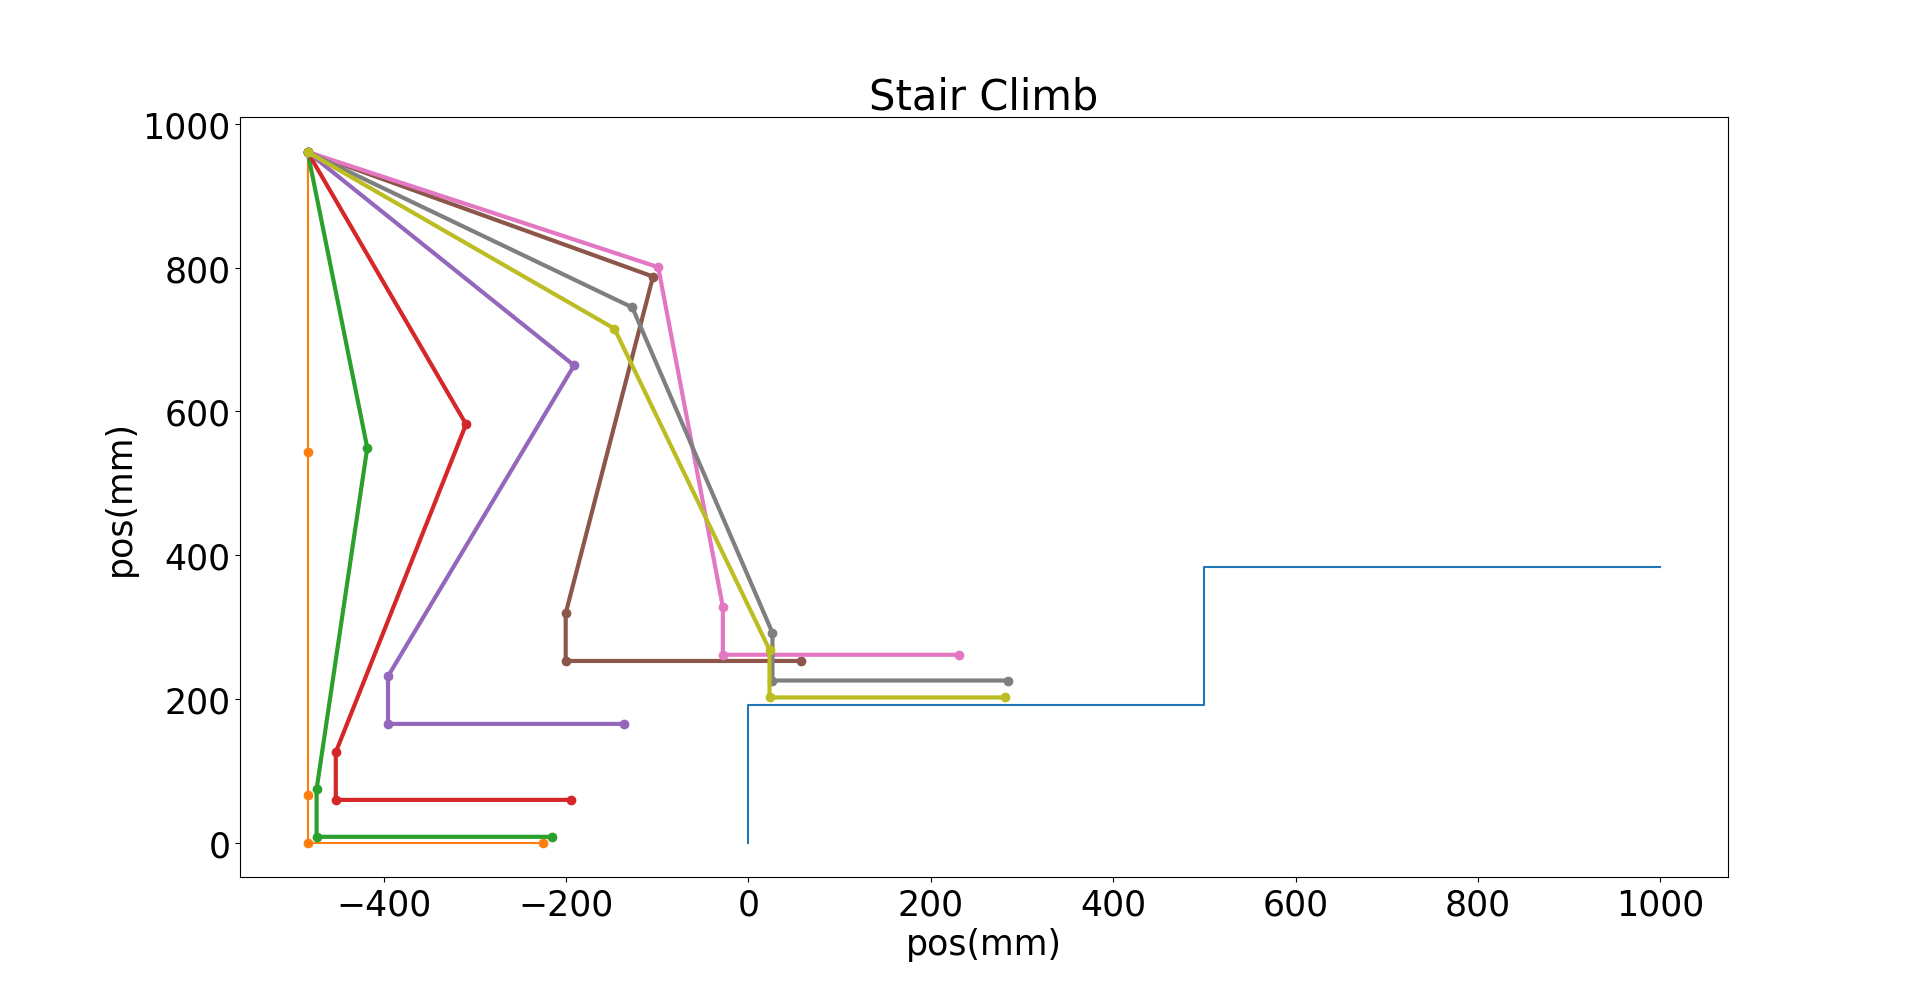
\includegraphics[scale=0.20]{images/stairs_climb.png}
%     \caption{The leg motion over the stepping trajectory while keeping the ankle parallel with the ground. Inverse kinematics was then used to solve for the joint angles.}
%     \label{fig:stairsclimbing}
% \end{figure}

\begin{figure}[h!]
  \centering 
  \begin{subfigure}{\linewidth} 
    \centering
    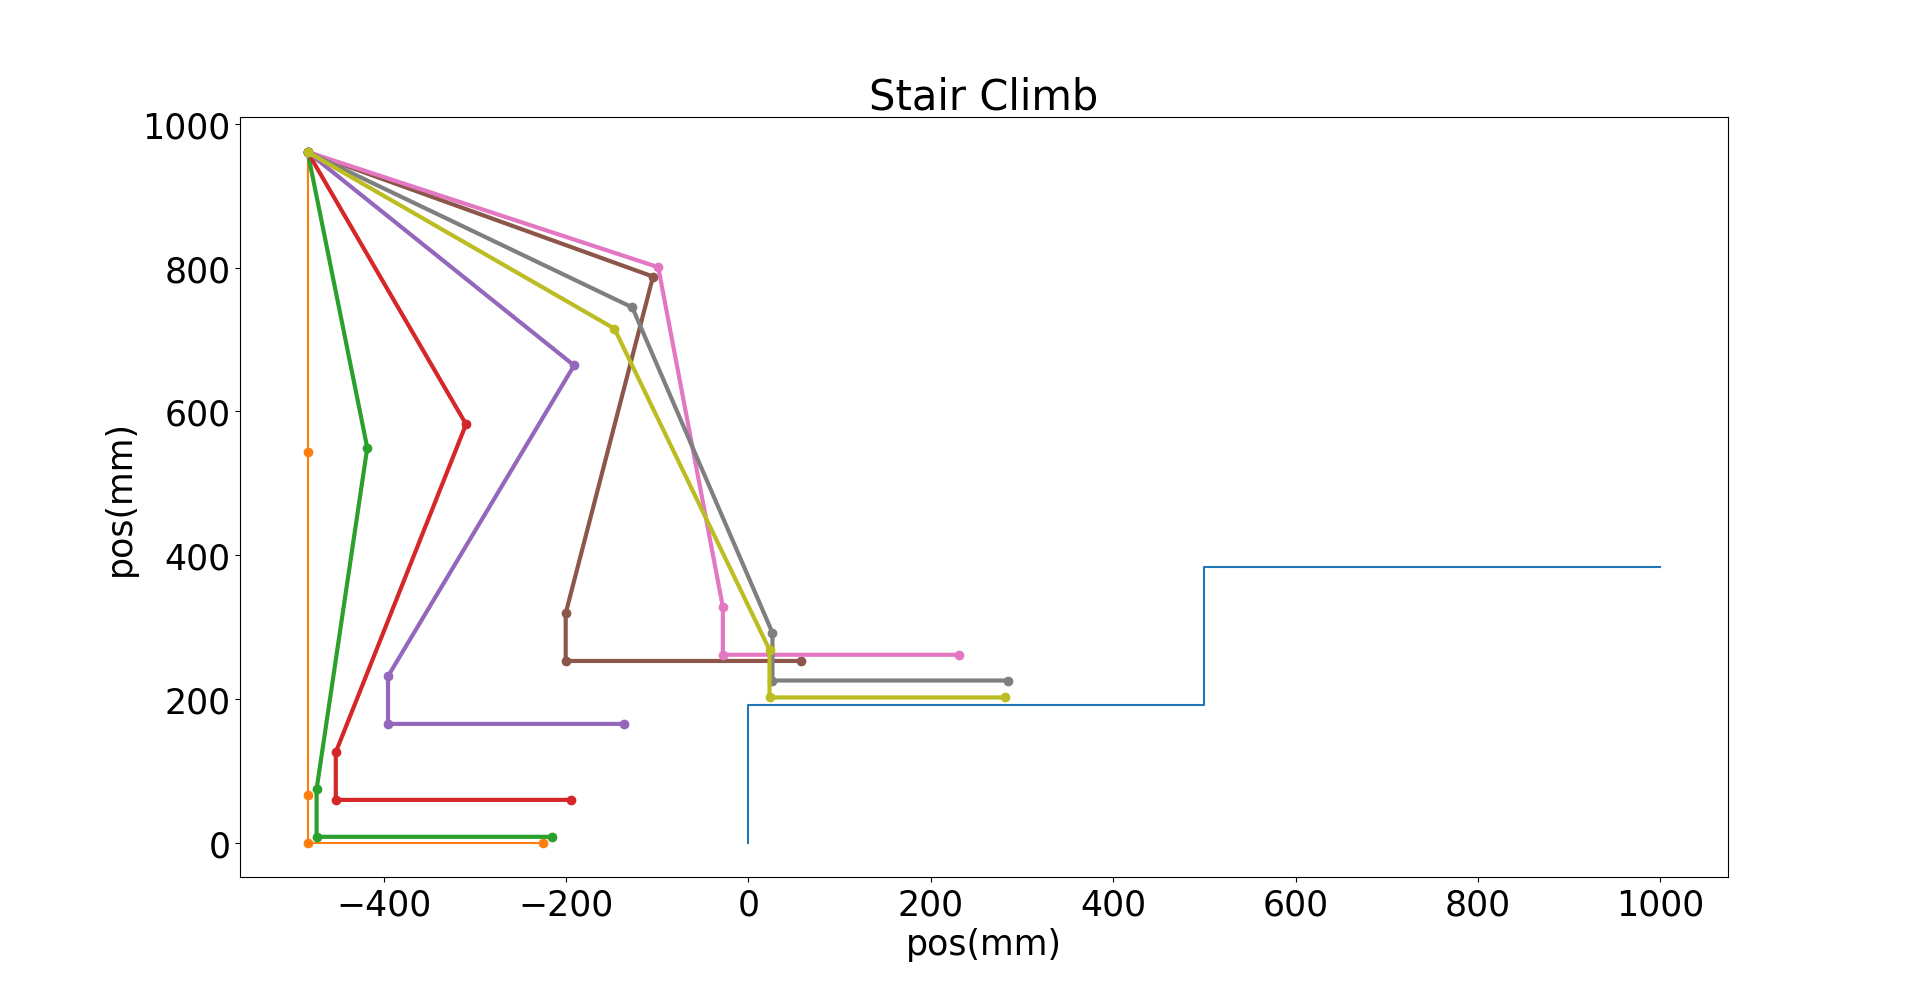
\includegraphics[scale=0.20]{images/stairs_climb.png}
    \caption{The leg motion over the stepping trajectory while keeping the ankle parallel with the ground. Inverse kinematics was then used to solve for the joint angles.}
    \label{fig:stairsclimbing}
  \end{subfigure} 
    \begin{subfigure}{\linewidth} 
    \centering 
    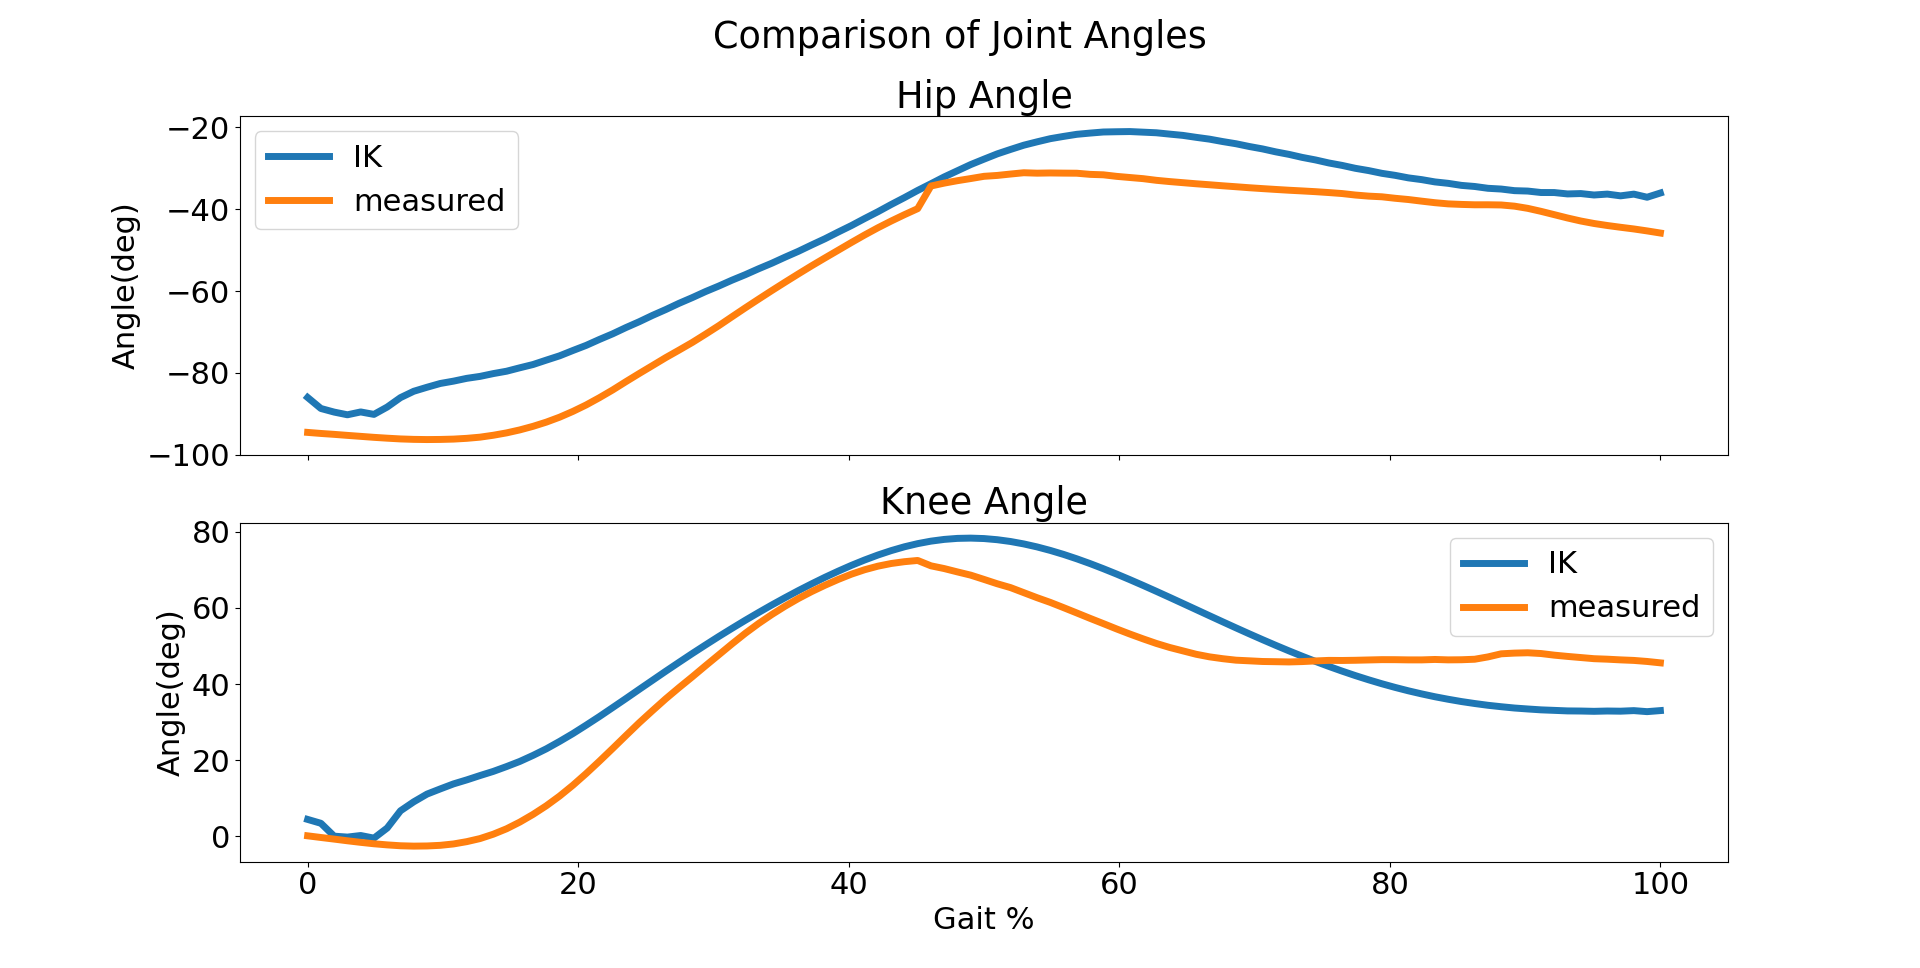
\includegraphics[ scale=0.20]{images/joint_angle_stairs_no_ankle.png} 
    \caption{Comparison of the joint angle. The IK path was calculated using the inverse kinematics and the toe tip. The measured joint angles are independently measured using the Vicon tracking software.}  
    \label{fig:config3} 
  \end{subfigure}   
  \caption{Control of the leg from the ground to the first step. The joint angle are calculated and compared to the measured joint angles. } 
  \label{fig:singleSubject} 
\end{figure}   

% \begin{figure}
%     \centering 
%     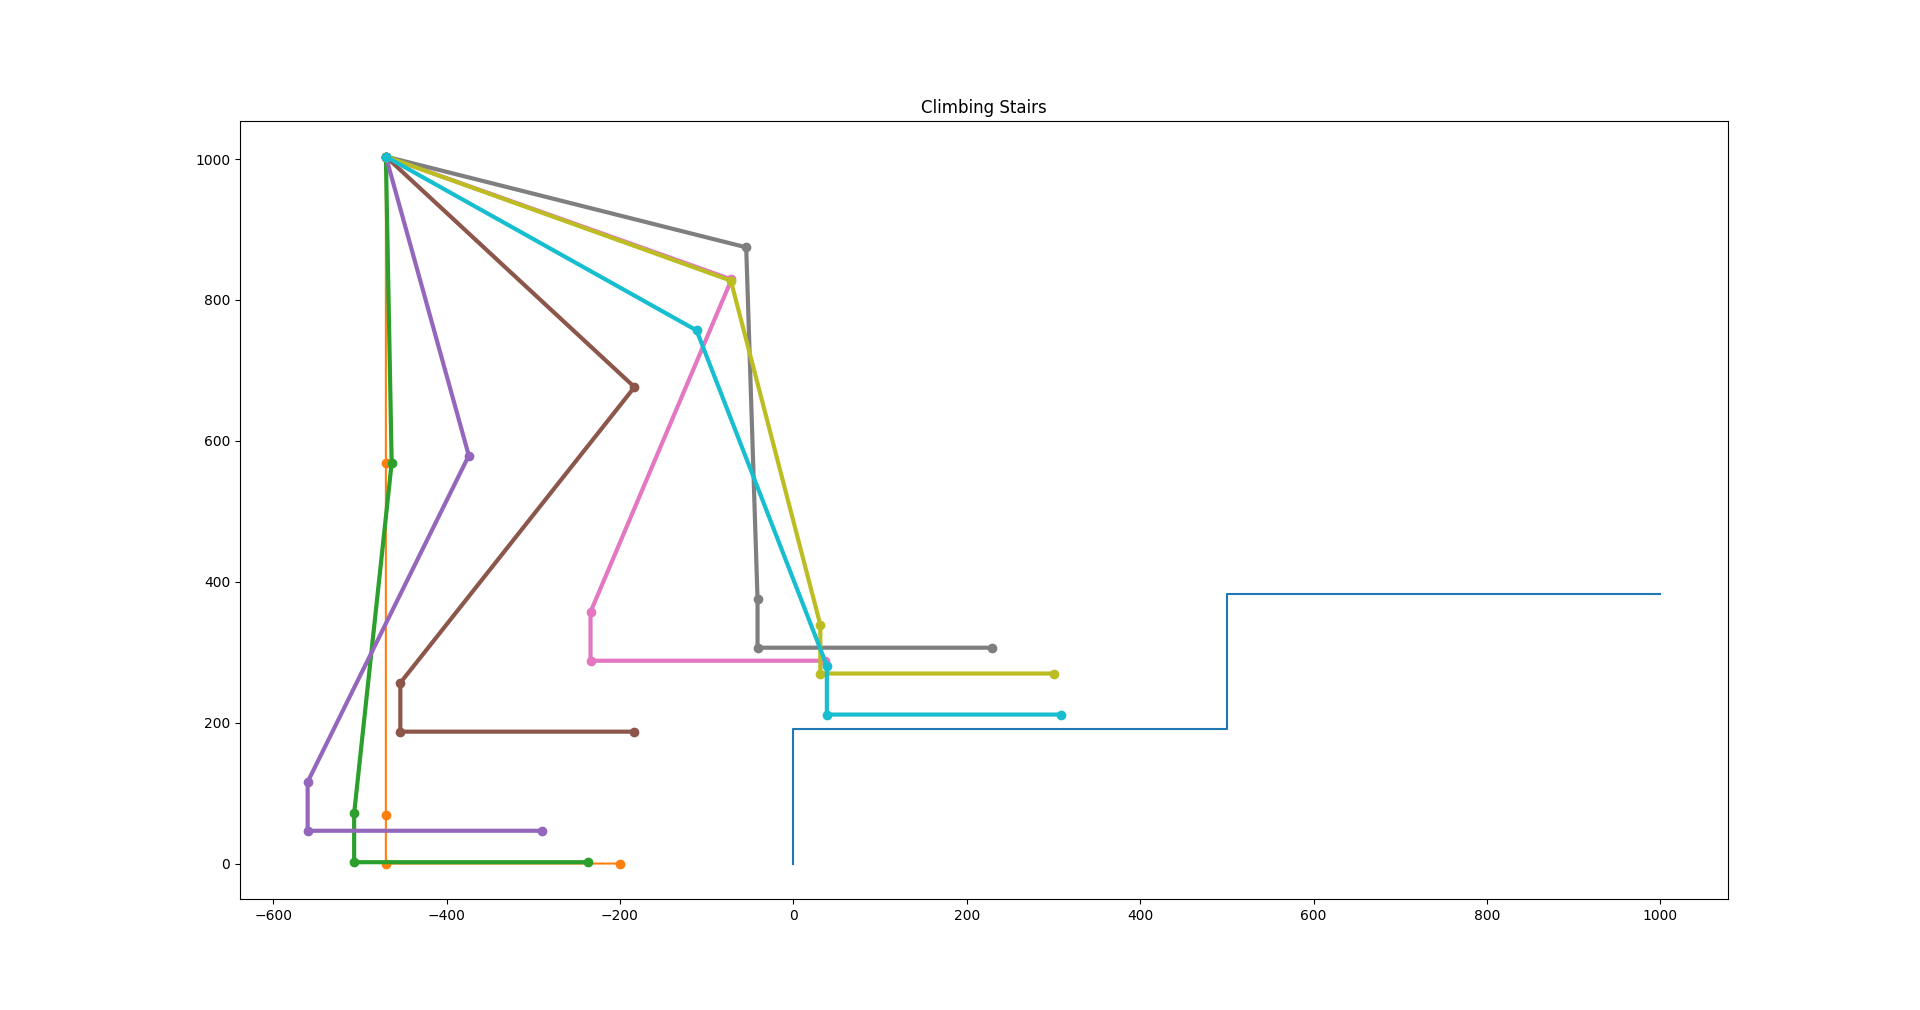
\includegraphics[frame, scale=0.16]{images/climbing_stair.png} 
%     \caption{The leg motion over the stepping trajectory while keeping the ankle parallel with the ground. Inverse kinematics was then used to solve for the joint angles.} 
%     \label{fig:stairsclimbing} 
% \end{figure} 

